%%%%%%%%%%%%%%%%%%%%%%%%%%%%%%%%%%%%%%%%%%%%%%%%%%%%%%%%%%%%%%%%%%%%%
%% Supporting Information
%% Optical Thermometry in Monolayer WS2: Raman and PL Spectroscopy, 5 K to 1273 K
%% Draft v1 — G. Lee
%%%%%%%%%%%%%%%%%%%%%%%%%%%%%%%%%%%%%%%%%%%%%%%%%%%%%%%%%%%%%%%%%%%%%
\documentclass[letterpaper]{article}

\usepackage[T1]{fontenc}
\usepackage[utf8]{inputenc}

\usepackage{geometry}
\geometry{margin=1in}

\usepackage{graphicx}
\usepackage{xcolor}
\usepackage{soul}
% Revision highlight for FC review; to remove, redefine as \newcommand{\rev}[1]{#1}
\definecolor{revgreen}{RGB}{160,255,160}
\sethlcolor{revgreen}
\DeclareRobustCommand{\rev}[1]{\hl{#1}}
\usepackage{float}
\usepackage{amsmath}
\usepackage{booktabs}
\usepackage{array}

\usepackage{chemformula}
\usepackage[version=4]{mhchem}

\usepackage[style=chem-acs]{biblatex}
\addbibresource{references.bib}

% SI figure numbering: S1, S2, ...
\renewcommand{\thefigure}{S\arabic{figure}}
\setcounter{figure}{0}
\renewcommand{\thetable}{S\arabic{table}}
\setcounter{table}{0}

\usepackage{authblk}
\author[1]{G. Lee}
\author[1]{A. Borel}
\author[2]{T. Taniguchi}
\author[3]{K. Watanabe}
\author[1]{F. Sirotti}
\author[1]{F. Cadiz}

\affil[1]{Laboratoire de Physique de la Matière Condensée, CNRS,
Ecole polytechnique, Institut Polytechnique de Paris, 91120 Palaiseau, France}
\affil[2]{International Center for Materials Nanoarchitectonics, National Institute for
Materials Science, 1-1 Namiki, Tsukuba 305-0044, Japan}
\affil[3]{Research Center for Functional Materials, National Institute for Materials
Science, 1-1 Namiki, Tsukuba 305-0044, Japan}

\title{Supporting Information\\[0.3em]
Optical Thermometry in Monolayer \ce{WS2}: Raman and
Photoluminescence Spectroscopy from 5~K to 1273~K}

\date{*Email: fabian.cadiz@polytechnique.edu}

\begin{document}

\maketitle

%%%%%%%%%%%%%%%%%%%%%%%%%%%%%%%%%%%%%%%%%%%%%%%%%%%%%%%%%%%%%%%%%%%%%
\section*{S1. Raman: Individual (E$^1_{2g}$, 2LA) versus Merged-Peak Fitting}
%%%%%%%%%%%%%%%%%%%%%%%%%%%%%%%%%%%%%%%%%%%%%%%%%%%%%%%%%%%%%%%%%%%%%

In addition to the A$_{1g}$($\Gamma$) mode used as the primary thermometer in
the main text, the E$^1_{2g}$($\Gamma$) and 2LA(M) modes ($\sim$351 and
$\sim$347~cm$^{-1}$ at room temperature, respectively) were tracked as a
function of temperature for both samples. These two modes sit only
$\sim$5~cm$^{-1}$ apart at room temperature and broaden and redshift with
increasing temperature, so that they progressively overlap and become
difficult to resolve individually. Each dataset was fitted \rev{in two ways}: (i) as
two independent Lorentzian peaks (individual fit), and (ii) as a single
Lorentzian standing in for the unresolved pair (merged fit).

\textbf{Non-encapsulated sample.} Figure~\ref{fig:s1}(a,b) shows the
individually-fitted E$^1_{2g}$ and 2LA positions versus temperature. Both
peaks are well resolved and the individual fits are stable across the full
range; linear fits restricted to $T \geq 600$~K give slopes of
$-0.0174~\mathrm{cm^{-1}/K}$ (E$^1_{2g}$) and $-0.0137~\mathrm{cm^{-1}/K}$
(2LA). Figure~\ref{fig:s1}(c) shows the merged-peak fit, which is flatter
below $\sim$500~K and only becomes clearly linear at higher temperature; a
linear fit restricted to $T \geq 500$~K yields
$-0.0179 \pm 0.0002~\mathrm{cm^{-1}/K}$ ($R^2 = 0.998$, $n = 15$) -- consistent
with the individual-peak slopes, since the non-encapsulated sample's
individual fits are already well-behaved.

\textbf{hBN-encapsulated sample.} Figure~\ref{fig:s1}(d,e) shows that the
individual fit is far less reliable for this sample: above $\sim$900~K, the
optimizer is prone to bound-splitting artifacts and chain-drift, and the
E$^1_{2g}$ position visibly deviates from a physical monotonic redshift (it
even turns upward in Fig.~\ref{fig:s1}(d)), with error bars several times
larger than at low temperature. This motivates treating E$^1_{2g}$ and 2LA
as a single merged Lorentzian peak for this sample
(Figure~\ref{fig:s1}(f)), which gives a more stable, if less precise,
position estimate. A pooled linear fit over \rev{$T \geq 250$~K, below which the merged position
does not decrease with temperature} (combining all
four measurement stages: LT, cooldown, 1st heat-up, 2nd heat-up) yields a
slope of \rev{$-0.0114 \pm 0.0007~\mathrm{cm^{-1}/K}$ ($R^2 = 0.915$, $n = 24$)},
consistent in sign and order of magnitude with the non-encapsulated result.

This fit should not, however, be read as a quantitative calibration for the
encapsulated sample. Three features of the data argue against it. First, the
intensity redistribution described in the main text removes the doublet
entirely between $\sim$373~K and $\sim$923~K, so the fit spans a 550~K gap and
is effectively constrained by two separated clusters of points rather than by
a continuous trend. Second, below $\sim$400~K the merged position is not
monotonic: it rises from $349.1$ to $350.9~\mathrm{cm^{-1}}$ between 5~K and
293~K before decreasing again. Third, repeated acquisitions at the same
nominal temperature differ by up to $2.3~\mathrm{cm^{-1}}$ at high
temperature, several times the corresponding fit uncertainty
($\sim$0.4~cm$^{-1}$), indicating that the merged position is not reproducible
at that level.

The E$^1_{2g}$+2LA doublet is therefore used only as a qualitative,
sign-and-order-of-magnitude check. For the non-encapsulated sample it provides
a usable secondary indicator above $\sim$500~K; for the encapsulated sample no
quantitative slope is claimed. In neither case is it proposed as a thermometer
in place of the A$_{1g}$ mode used in the main text.

\begin{figure}[H]
  \centering
  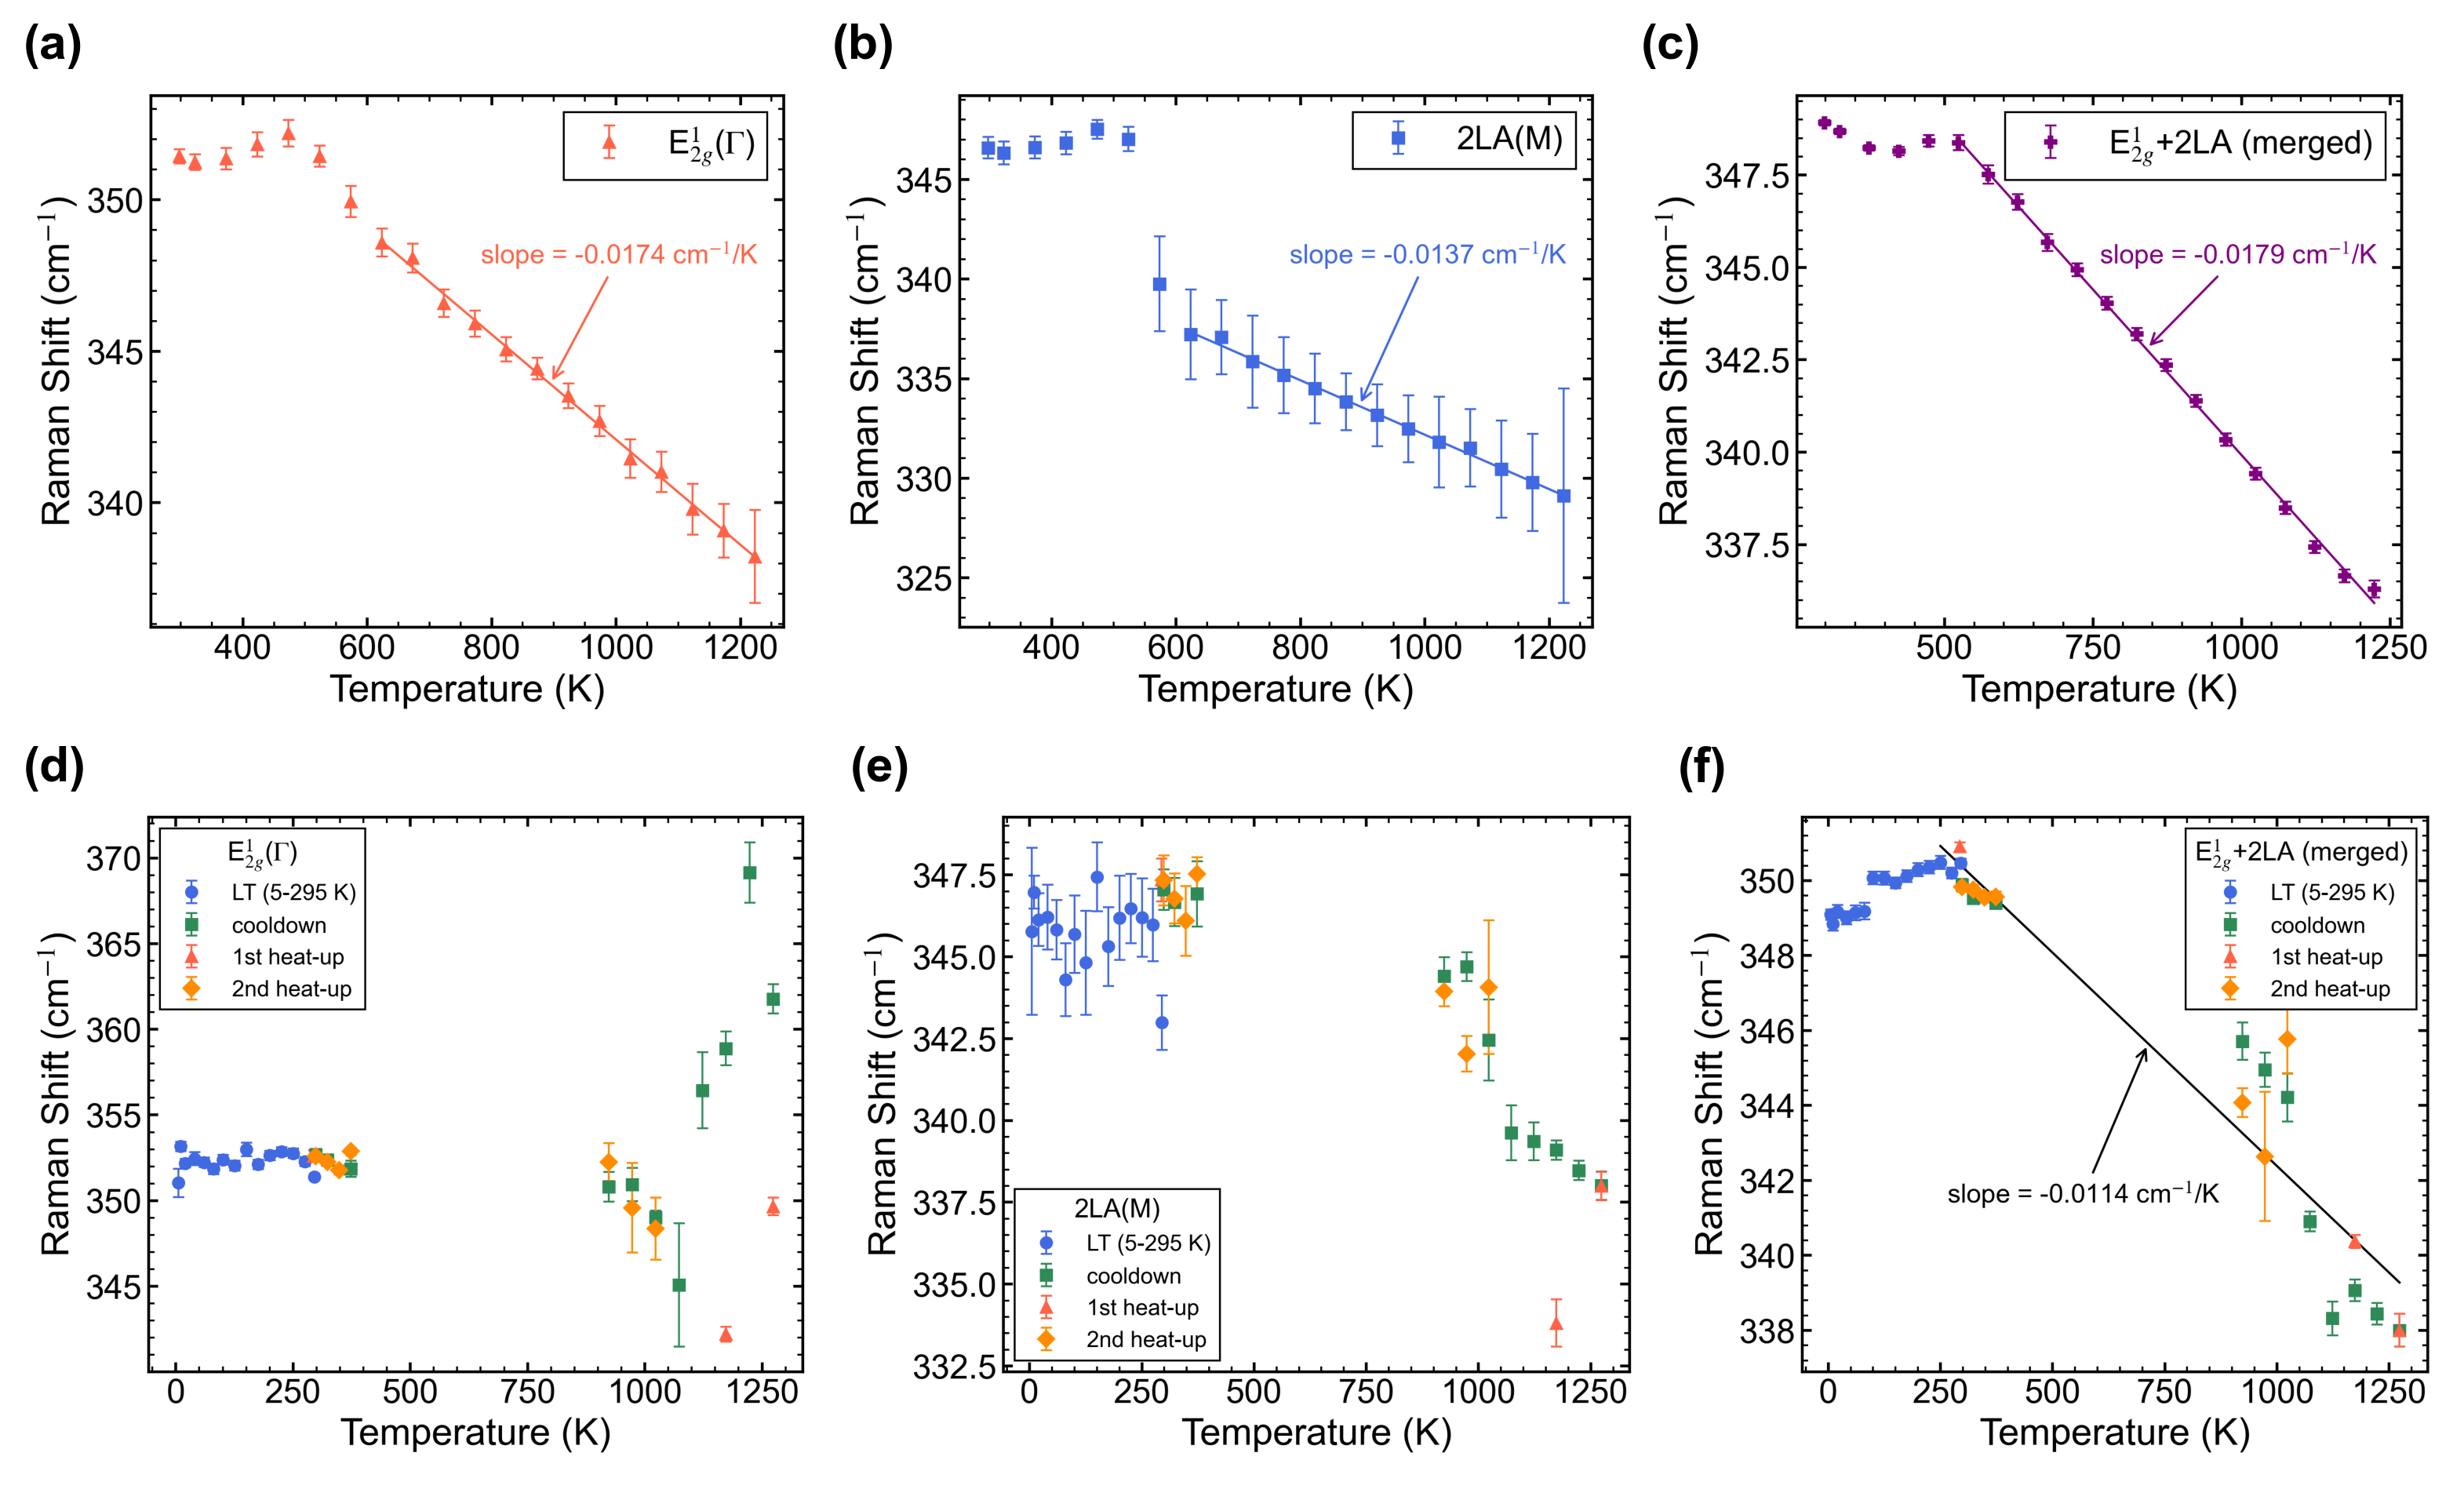
\includegraphics[width=\linewidth]{Figures/figS1.png}
  \caption{Individual versus merged-peak fitting of the E$^1_{2g}$+2LA
    doublet. Top row: non-encapsulated sample -- (a) E$^1_{2g}$ individual
    fit, (b) 2LA individual fit, (c) merged-peak fit ($T \geq 500$~K linear
    fit shown). Bottom row: hBN-encapsulated sample -- (d) E$^1_{2g}$
    individual fit, (e) 2LA individual fit, both showing instability above
    $\sim$900~K, (f) merged-peak fit, pooled linear fit over
    \rev{$T \geq 250$~K} across all four measurement stages.}
  \label{fig:s1}
\end{figure}

%%%%%%%%%%%%%%%%%%%%%%%%%%%%%%%%%%%%%%%%%%%%%%%%%%%%%%%%%%%%%%%%%%%%%
\section*{S2. Temperature-Dependent Raman Spectra of hBN-Encapsulated \ce{WS2}}
%%%%%%%%%%%%%%%%%%%%%%%%%%%%%%%%%%%%%%%%%%%%%%%%%%%%%%%%%%%%%%%%%%%%%

Figure~\ref{fig:s2} shows the Raman spectra of the hBN-encapsulated \ce{WS2}
monolayer over the full measured temperature range, combining the low-temperature
(5~K to 295~K) and high-temperature (RT to \rev{1273~K}) datasets.
Data points where the peak position could not be reliably extracted are excluded
from the analysis. \rev{The A$_{1g}$ positions from the cooldown and the two
heat-up stages scatter around the same line} (Figure~\ref{fig:s2}(b))\rev{, with
stage-to-stage differences of up to $\sim$0.8~cm$^{-1}$ but no consistent
offset between heating and cooling.}

\begin{figure}[H]
  \centering
  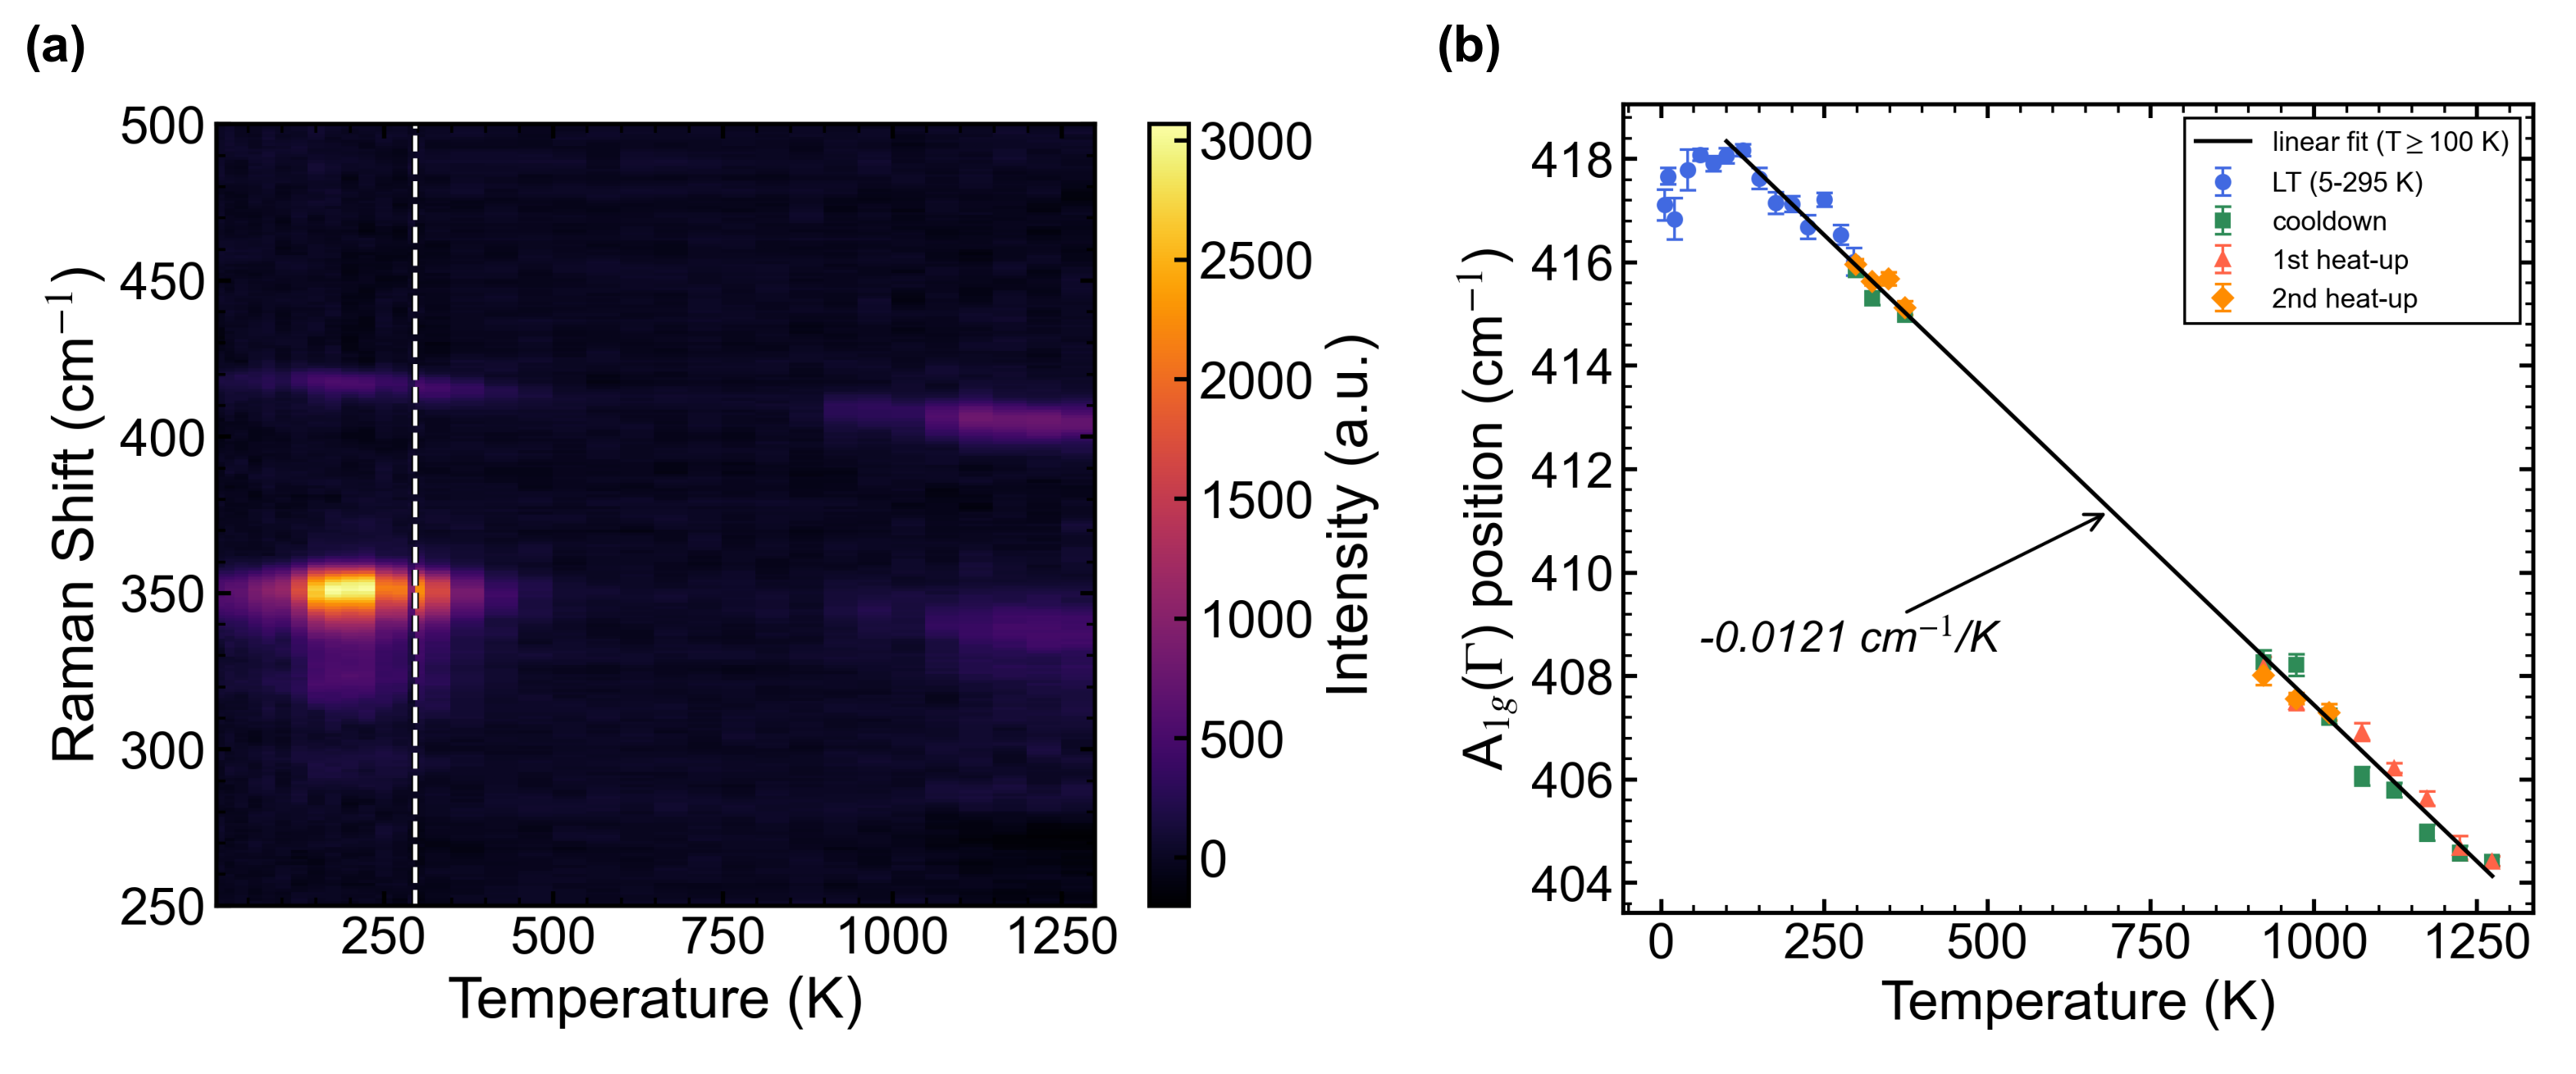
\includegraphics[width=\linewidth]{Figures/figS2.png}
  \caption{\rev{Temperature-dependent Raman response of the hBN-encapsulated}
    \ce{WS2} \rev{monolayer. (a) Two-dimensional map of Raman intensity versus
    temperature (5--1273~K) and Raman shift; the dashed line marks the
    boundary between the cryostat (5~K--RT) and micro-heater (RT--1273~K)
    stages. (b) A$_{1g}$ peak position versus temperature for each
    measurement stage. The solid line is a linear fit to this sample over
    $T \geq 100$~K ($-0.0121$~cm$^{-1}$/K), as used in the main text; cooldown
    and heat-up data scatter around the same line.}}
\label{fig:s2}
\end{figure}

%%%%%%%%%%%%%%%%%%%%%%%%%%%%%%%%%%%%%%%%%%%%%%%%%%%%%%%%%%%%%%%%%%%%%
\section*{S3. Comparison of Bandgap Temperature Models}
%%%%%%%%%%%%%%%%%%%%%%%%%%%%%%%%%%%%%%%%%%%%%%%%%%%%%%%%%%%%%%%%%%%%%

Three empirical and semi-empirical models for the temperature dependence of
the bandgap energy were fitted to the neutral-exciton peak energy $E_0(T)$
extracted from Voigt fits of the PL spectra. The main text uses the Pässler
model (Eq.~2); the two alternative models below are compared against it here.

\textbf{Varshni model (1967) \cite{varshni-1967}:}
\begin{equation}
E(T) = E_0 - \frac{\alpha T^2}{T + \beta},
\end{equation}
where $E_0$ is the zero-temperature bandgap, $\alpha$ is the
electron--phonon coupling constant (eV/K), and $\beta$ is an effective Debye
temperature (K). This model is purely empirical and does not reduce to the
correct zero-temperature curvature.

\textbf{O'Donnell--Chen model (1991) \cite{odonnell-1991}:}
\begin{equation}
E(T) = E_0 - S \hbar\omega
\left[ \coth\!\left(\frac{\hbar\omega}{2 k_B T}\right) - 1 \right],
\end{equation}
where $S$ is a dimensionless Huang--Rhys-like electron--phonon coupling
strength and $\hbar\omega$ is the mean phonon energy. At high temperature this
model is linear in $T$, with slope $2 S k_B$.

Figure~\ref{fig:s3} shows all three model fits (Pässler included for
reference) to the data together with the corresponding residuals. The fitted
parameters and goodness-of-fit metrics are summarized in
Table~\ref{tab:s1}. The Varshni model systematically overestimates the
energy at low temperature, while both the Pässler and O'Donnell--Chen
models -- which share the same physically-motivated saturation to a
temperature-independent phonon population at low $T$ -- reproduce the data
to within the experimental uncertainty over the full range.

\begin{figure}[H]
  \centering
  \begin{minipage}{0.48\linewidth}
    \centering
    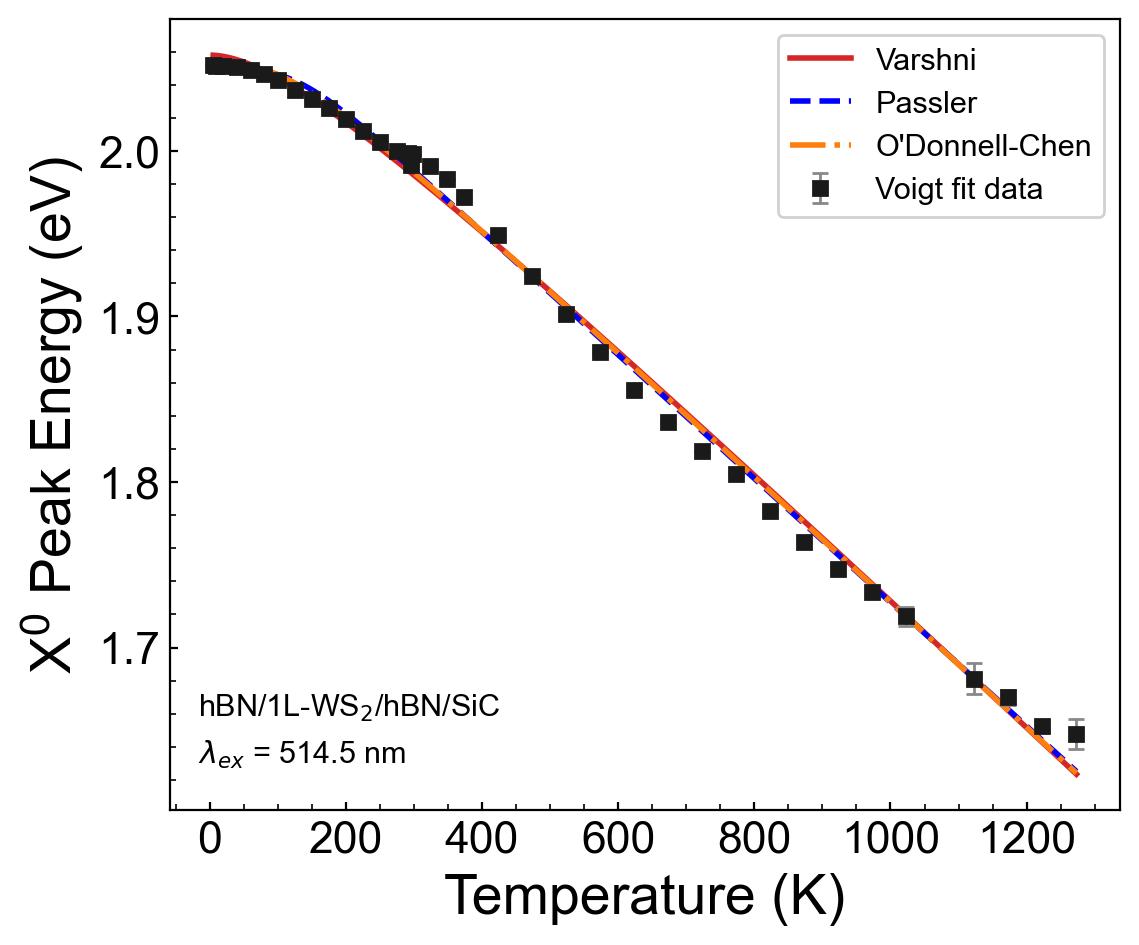
\includegraphics[width=\linewidth]{Figures/figS3a_E0_model_combined.png}
    \\ (a)
  \end{minipage}
  \hfill
  \begin{minipage}{0.48\linewidth}
    \centering
    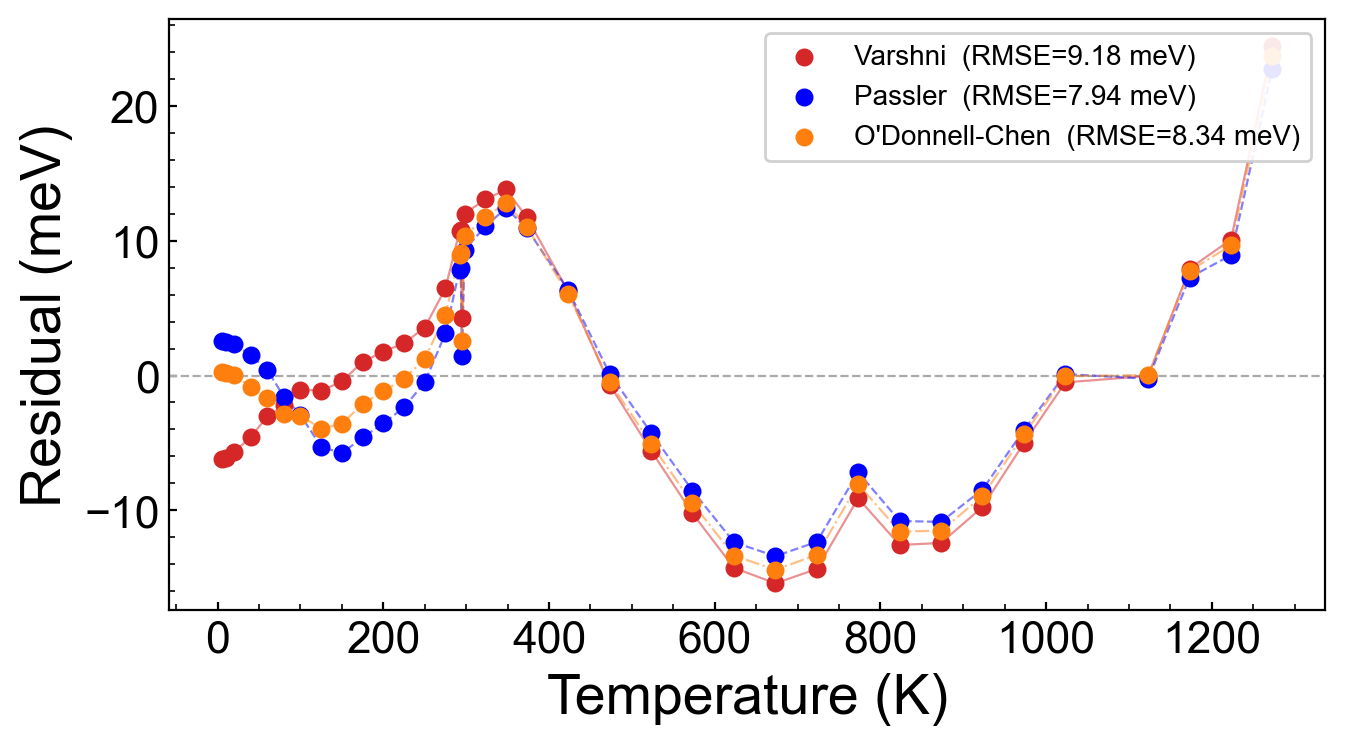
\includegraphics[width=\linewidth]{Figures/figS3b_E0_model_residuals.png}
    \\ (b)
  \end{minipage}
  \caption{Comparison of bandgap temperature models fitted to the
    neutral-exciton peak energy of hBN-encapsulated \ce{WS2}.
    (a) Experimental $E_0(T)$ (symbols) and fits using the Varshni
    (dashed red), Pässler (solid blue), and O'Donnell--Chen (dash-dot orange)
    models.
    (b) Fit residuals (data $-$ model) in meV for each model, showing that the
    Varshni model systematically overestimates the energy at low temperature,
    while both the Pässler and O'Donnell--Chen models fit the data to within the
    experimental uncertainty over the full range.}
  \label{fig:s3}
\end{figure}

\begin{table}[H]
  \centering
  \caption{Fitted parameters and goodness-of-fit metrics for the three
    bandgap temperature models (weighted least-squares fit to the
    neutral-exciton $X_A^0$ peak energy).}
  \label{tab:s1}
  % Transposed (models as columns) so the table fits the text width.
  \begin{tabular}{lccc}
    \toprule
     & Varshni & Pässler & O'Donnell--Chen \\
    \midrule
    $E_0(0)$ (eV)             & $2.0578 \pm 0.0037$ & $2.0491 \pm 0.0036$ & $2.0514 \pm 0.0034$ \\
    $\alpha$ ($10^{-4}$ eV/K) & $3.908 \pm 0.116$   & $3.741 \pm 0.069$   & --- \\
    $\beta$ (K)               & $185.2 \pm 41.4$    & ---                 & --- \\
    $\Theta$ (K)              & ---                 & $280.1 \pm 28.8$    & --- \\
    $p$                       & ---                 & $4.04 \pm 2.23$     & --- \\
    $S$                       & ---                 & ---                 & $2.210 \pm 0.038$ \\
    $\hbar\omega$ (meV)       & ---                 & ---                 & $27.3 \pm 3.4$ \\
    \midrule
    $R^2$                     & 0.9952              & 0.9964              & 0.9961 \\
    RMSE (meV)                & 9.18                & 7.94                & 8.34 \\
    \bottomrule
  \end{tabular}
\end{table}

%%%%%%%%%%%%%%%%%%%%%%%%%%%%%%%%%%%%%%%%%%%%%%%%%%%%%%%%%%%%%%%%%%%%%
\section*{S4. Voigt Fitting Procedure and Quality Assessment}
%%%%%%%%%%%%%%%%%%%%%%%%%%%%%%%%%%%%%%%%%%%%%%%%%%%%%%%%%%%%%%%%%%%%%

\rev{At each temperature, the $X_A^0$ emission was fitted with a Voigt profile,
the convolution of a Gaussian of standard deviation $\sigma$ and a Lorentzian of
half-width $\gamma$, evaluated through the Faddeeva function $w(z)$:}

\begin{equation}
\label{eq:voigt}
V(E) = A\,\frac{\mathrm{Re}\,[w(z)]}{\sigma\sqrt{2\pi}}, \qquad
z = \frac{E - E_0 + i\gamma}{\sigma\sqrt{2}},
\end{equation}

\rev{plus a constant background $B$. Below 125~K, where $X_A^0$ is spectrally
isolated, a single Voigt profile was fitted within a $\pm$22~meV window centred
on the peak position obtained at the previous temperature. From 125~K upwards,
$X_A^0$ broadens into the lower-energy trion ($X^-$) emission, and the full
measured spectral window was fitted with two Voigt profiles ($X_A^0$ and $X^-$)
sharing a common background, with the $X^-$ amplitude constrained not to exceed
that of $X_A^0$. The Gaussian and Lorentzian widths are
$\Gamma_G = 2\sqrt{2\ln 2}\,\sigma$ and $\Gamma_L = 2\gamma$; the total FWHM
$\Gamma_V$ of the $X_A^0$ component was obtained numerically from the
half-maximum crossings of the fitted profile rather than from an approximate
closed-form expression.}

Figure~\ref{fig:s4} shows representative \rev{fits at twelve temperatures}
spanning the full range.

\begin{figure}[H]
  \centering
  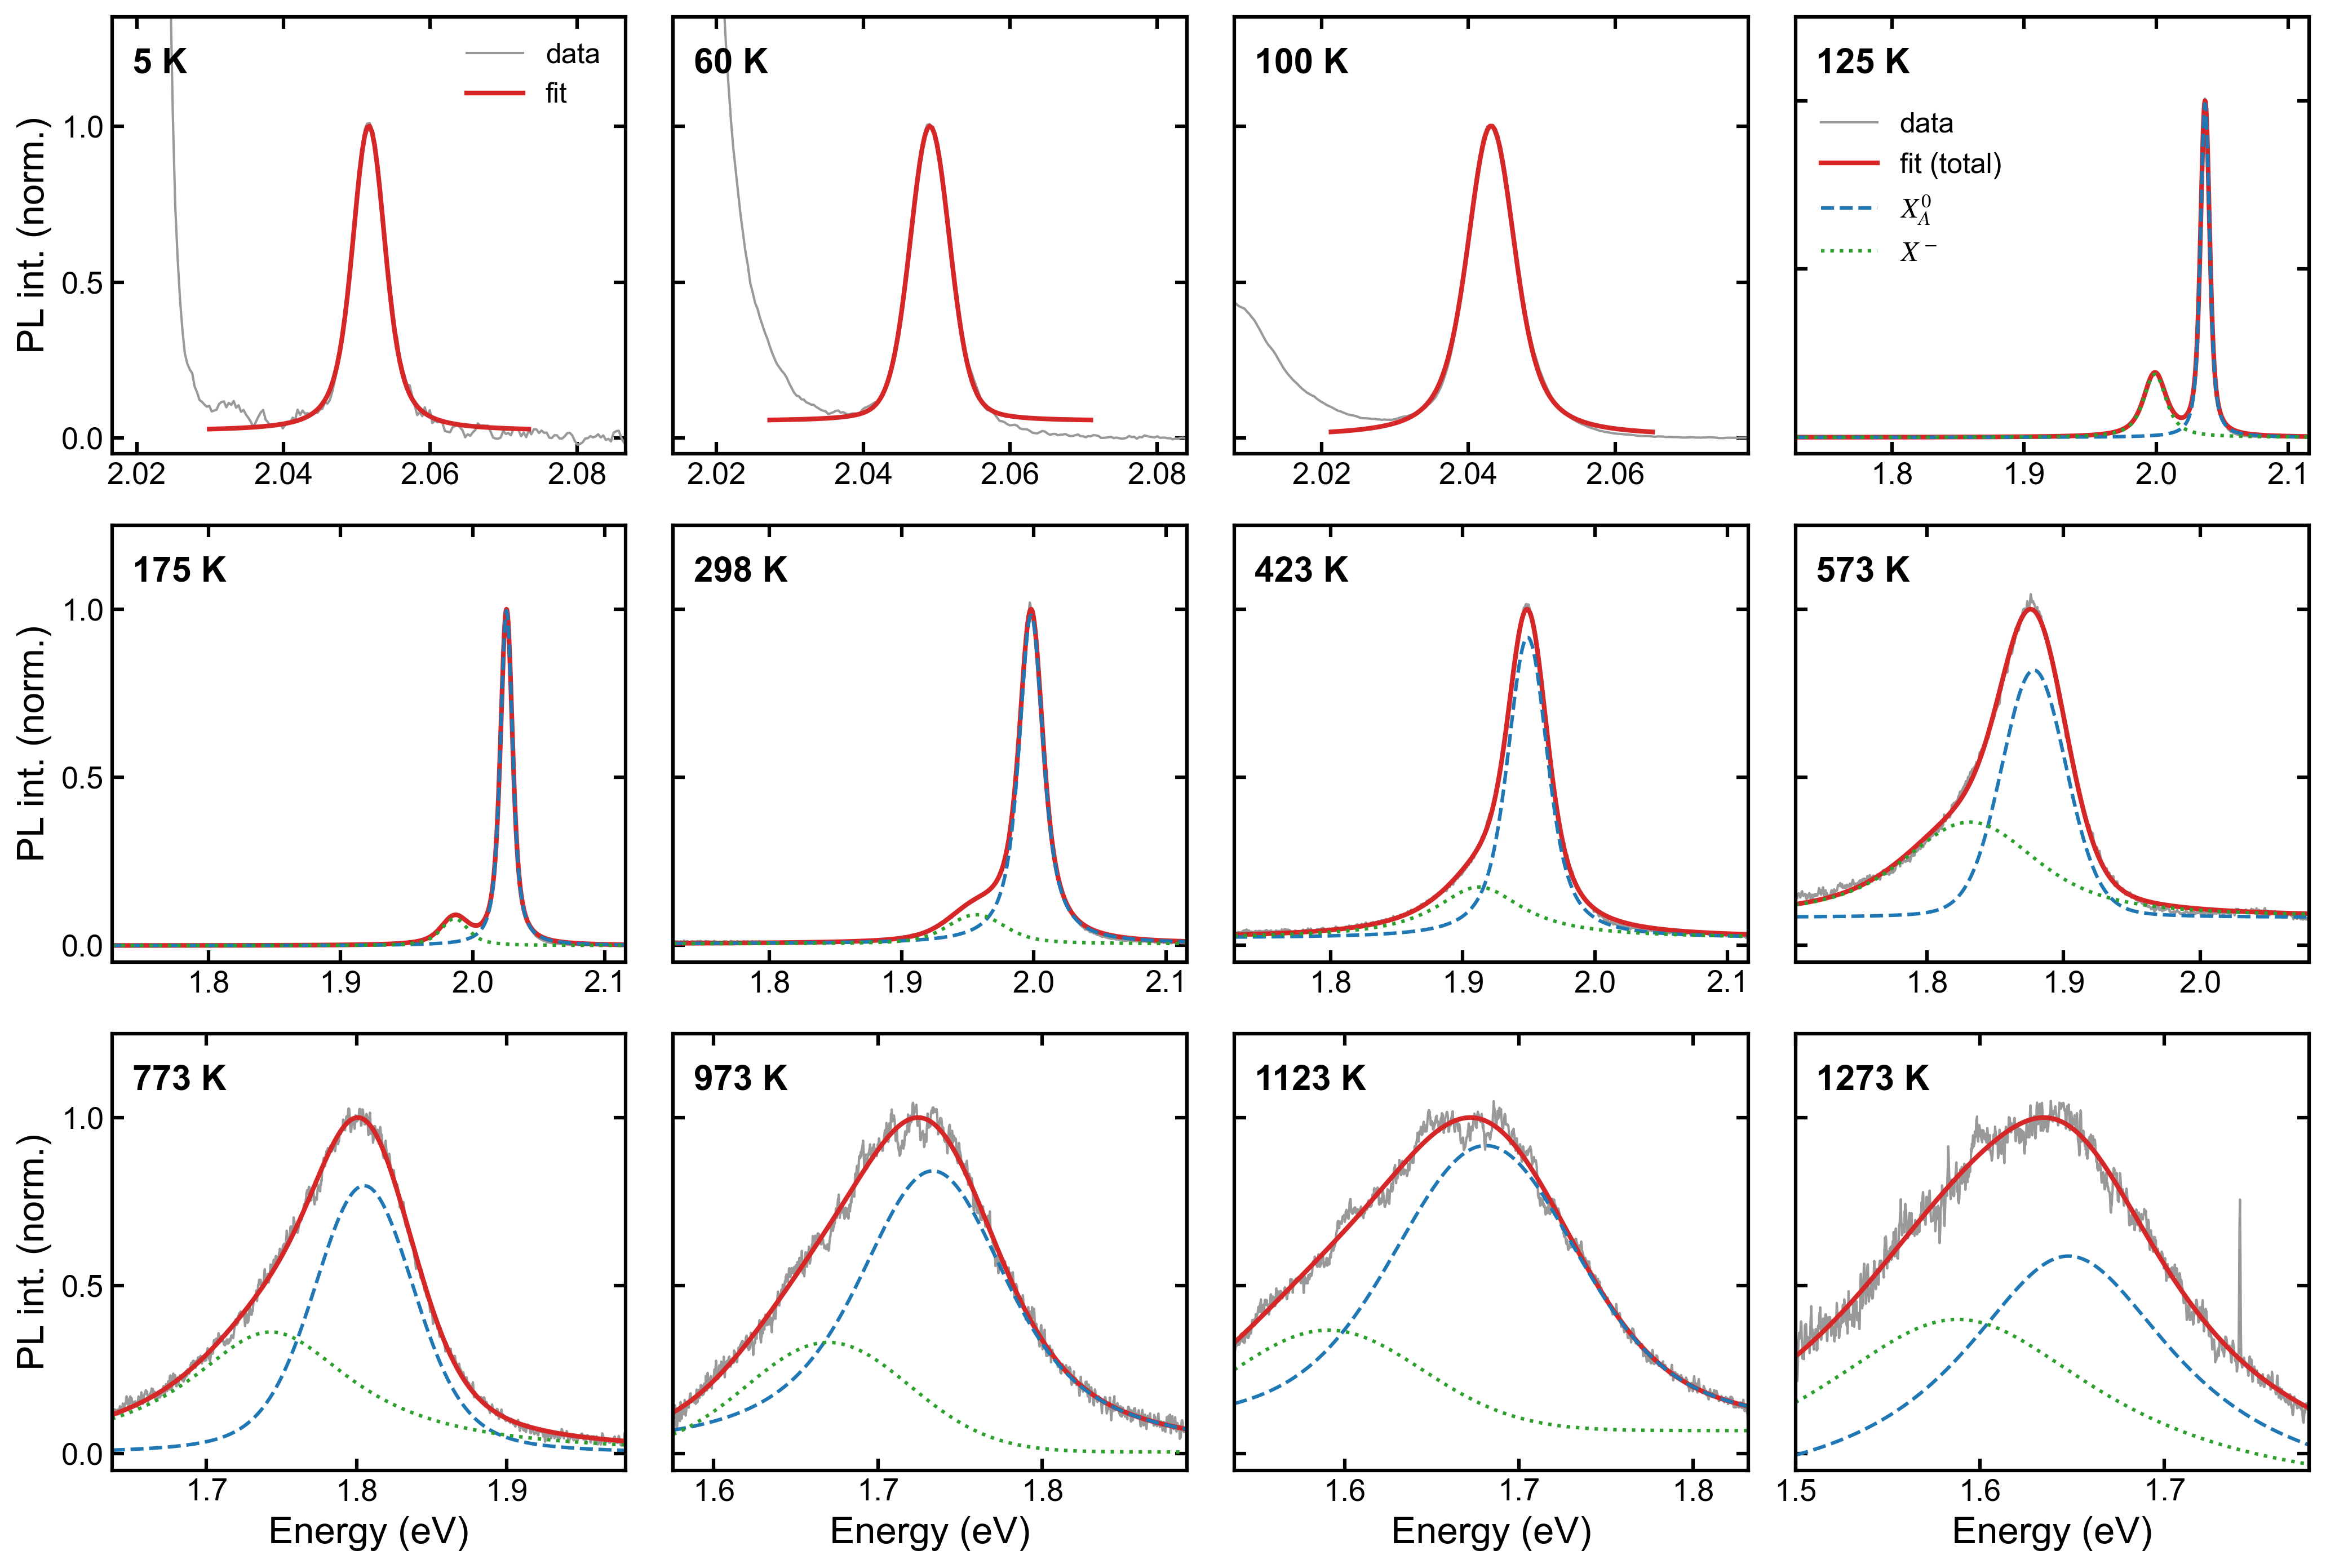
\includegraphics[width=\linewidth]{Figures/figS4.png}
  \caption{\rev{Representative Voigt fits to the PL spectra of hBN-encapsulated}
    \ce{WS2} \rev{at twelve temperatures. Grey: data; red: fit. Below 125~K (5, 60
    and 100~K) a single Voigt profile is fitted within $\pm$22~meV of $X_A^0$,
    and only this window is shown. From 125~K upwards the fit (red) is the sum
    of the $X_A^0$ (blue dashed) and $X^-$ (green dotted) components over the
    full acquisition window. Each panel is normalised to the maximum of the
    fit. At the highest temperatures the low-energy tail of the emission
    extends beyond the acquisition window.}}
\label{fig:s4}
\end{figure}

Note: the Gaussian and Lorentzian widths are strongly correlated in the fit,
and at several temperatures the optimizer converges to a bound, so that the
individual components are not reliably determined. Only the total Voigt
width is reported (Sec.~S5). The peak position $E_0$ is robust to this
degeneracy and all points are retained in the $E_0(T)$ dataset.

%%%%%%%%%%%%%%%%%%%%%%%%%%%%%%%%%%%%%%%%%%%%%%%%%%%%%%%%%%%%%%%%%%%%%
\section*{S5. Photoluminescence Linewidth and Integrated Intensity}
%%%%%%%%%%%%%%%%%%%%%%%%%%%%%%%%%%%%%%%%%%%%%%%%%%%%%%%%%%%%%%%%%%%%%

Figure~\ref{fig:s5}(a) shows the total Voigt FWHM $\Gamma_V$ of the $X_A^0$
emission as a function of temperature. The linewidth increases monotonically
from $\sim$5.3~meV at 5~K to $\sim$140~meV at 1273~K, consistent with an
increasing phonon-scattering-limited dephasing rate. \rev{Over 5--1000~K the linewidth
is well described by the phonon-scattering model
$\Gamma(T) = \Gamma_0 + c_1 T + c_2/[\exp(\Omega/k_BT) - 1]$}
\cite{selig-2016,moody-2015}\rev{, in which the linear term accounts for
acoustic phonons and the last term for optical phonons of mean energy $\Omega$.
The fit gives $\Gamma_0 = 5.5 \pm 1.0$~meV and $\Omega = 46 \pm 7$~meV, close
to the E$^1_{2g}$ and A$_{1g}$ phonon energies of} \ce{WS2} \rev{($\sim$44 and
$\sim$51~meV), while $c_1 = 9 \pm 15~\mu$eV/K is consistent with zero. Above
$\sim$250~K the optical-phonon occupation grows nearly linearly with
temperature, so the linewidth is well approximated by a straight line. A
linear fit over 250--1000~K gives $0.129 \pm 0.002$~meV/K with an rms residual
of 1.7~meV, slightly smaller than that of the model over the same range
(1.9~meV); this linear relation is the thermometric indicator used in the main
text. Above $\sim$1100~K the width levels off as the low-energy tail of the
emission extends beyond the acquisition window} (Fig.~\ref{fig:s4})\rev{, and
these points are excluded from both fits.} The decomposition of
the \rev{Voigt} profile (Eq.~\ref{eq:voigt}, Sec.~S4) into its Gaussian
($\Gamma_G$) and Lorentzian ($\Gamma_L$) contributions is not reported here:
the two components are strongly correlated in the fit and are not
individually well determined over much of the temperature range.

Figure~\ref{fig:s5}(b) shows the integrated PL intensity of $X_A^0$. The
emission is weak below $\sim$40~K and then rises by roughly two orders of
magnitude up to $\sim$175~K. This behaviour is characteristic of
tungsten-based monolayer TMDs, in which the lowest-lying exciton state is
spin-forbidden (dark) and sits a few tens of meV below the bright state
\cite{zhang-2015,molas-2017}: at low temperature carriers relax into the
dark state and bright emission is quenched, while increasing temperature
thermally activates the bright-state population. Above $\sim$175~K the
intensity decreases again, consistent with thermally activated non-radiative
recombination \cite{korn-2011} and with the thermal escape of excitons from
the radiative window \cite{robert-2016}. Above $\sim$800~K the extracted intensity is
no longer a faithful measure of the emission strength, since the strongly
broadened peak extends beyond the low-energy edge of the fitting window
(1.50~eV) and its integrated area cannot be reliably determined. The peak
\emph{position} is unaffected by this truncation, since the emission
maximum remains well inside the fitting window at all temperatures.

\begin{figure}[H]
  \centering
  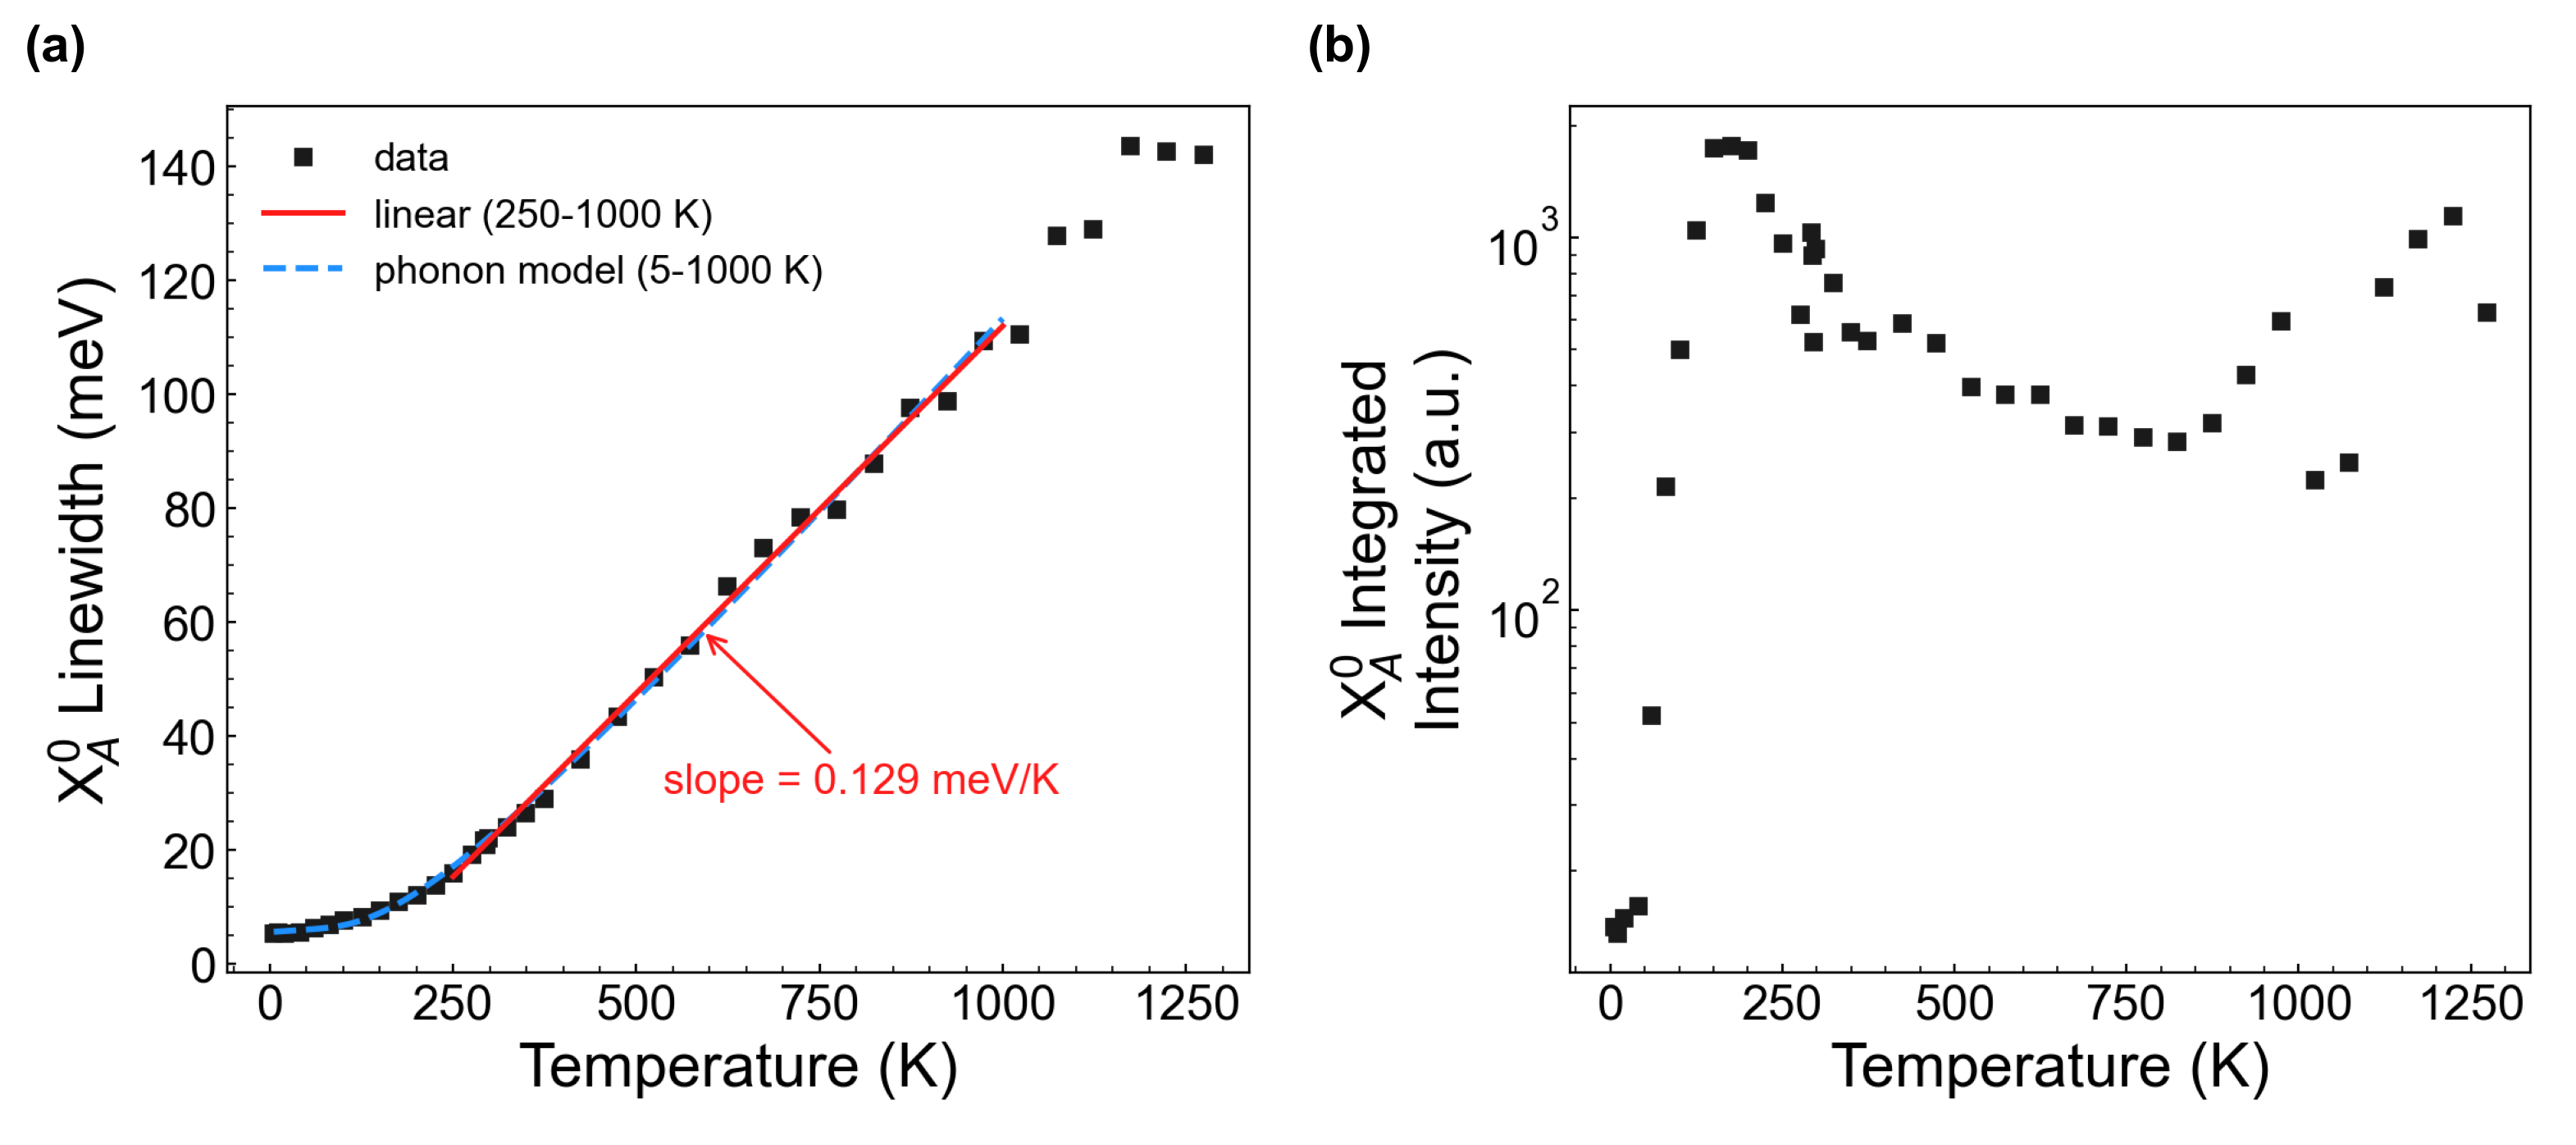
\includegraphics[width=\linewidth]{Figures/figS5.png}
  \caption{Temperature dependence of the PL linewidth and intensity.
    (a) Total Voigt FWHM $\Gamma_V$ of the $X_A^0$ emission versus
    temperature. \rev{Blue dashed line: phonon-scattering model fitted over
    5--1000~K; red line: linear fit over 250--1000~K.}
    (b) Integrated $X_A^0$ PL intensity versus temperature, showing the
    thermally activated rise from the dark-exciton ground state below
    $\sim$175~K and the subsequent thermal quenching at higher temperature.}
  \label{fig:s5}
\end{figure}

%%%%%%%%%%%%%%%%%%%%%%%%%%%%%%%%%%%%%%%%%%%%%%%%%%%%%%%%%%%%%%%%%%%%%
\section*{S6. Thermal Dissociation of \ce{WS2} Monolayer}
%%%%%%%%%%%%%%%%%%%%%%%%%%%%%%%%%%%%%%%%%%%%%%%%%%%%%%%%%%%%%%%%%%%%%

Figure~\ref{fig:s6} shows optical images of the non-encapsulated sample on the
SiC membrane before and after thermal treatment at 1000~$^\circ$C. After this
treatment no \ce{WS2} Raman signal was detectable, and the monolayer is absent
from the membrane under white-light illumination, consistent with thermal
dissociation through sulfur sublimation \cite{brainard-1968}. The
hBN-encapsulated sample, by contrast, remained intact after the same
treatment, with both Raman and PL still measurable at 1273~K. Thermal
dissociation therefore sets the practical upper bound for optical thermometry
on bare monolayers at $\sim$1273~K, while the encapsulated heterostructure was
limited here only by the operating range of the heater chip.

\begin{figure}[H]
  \centering
  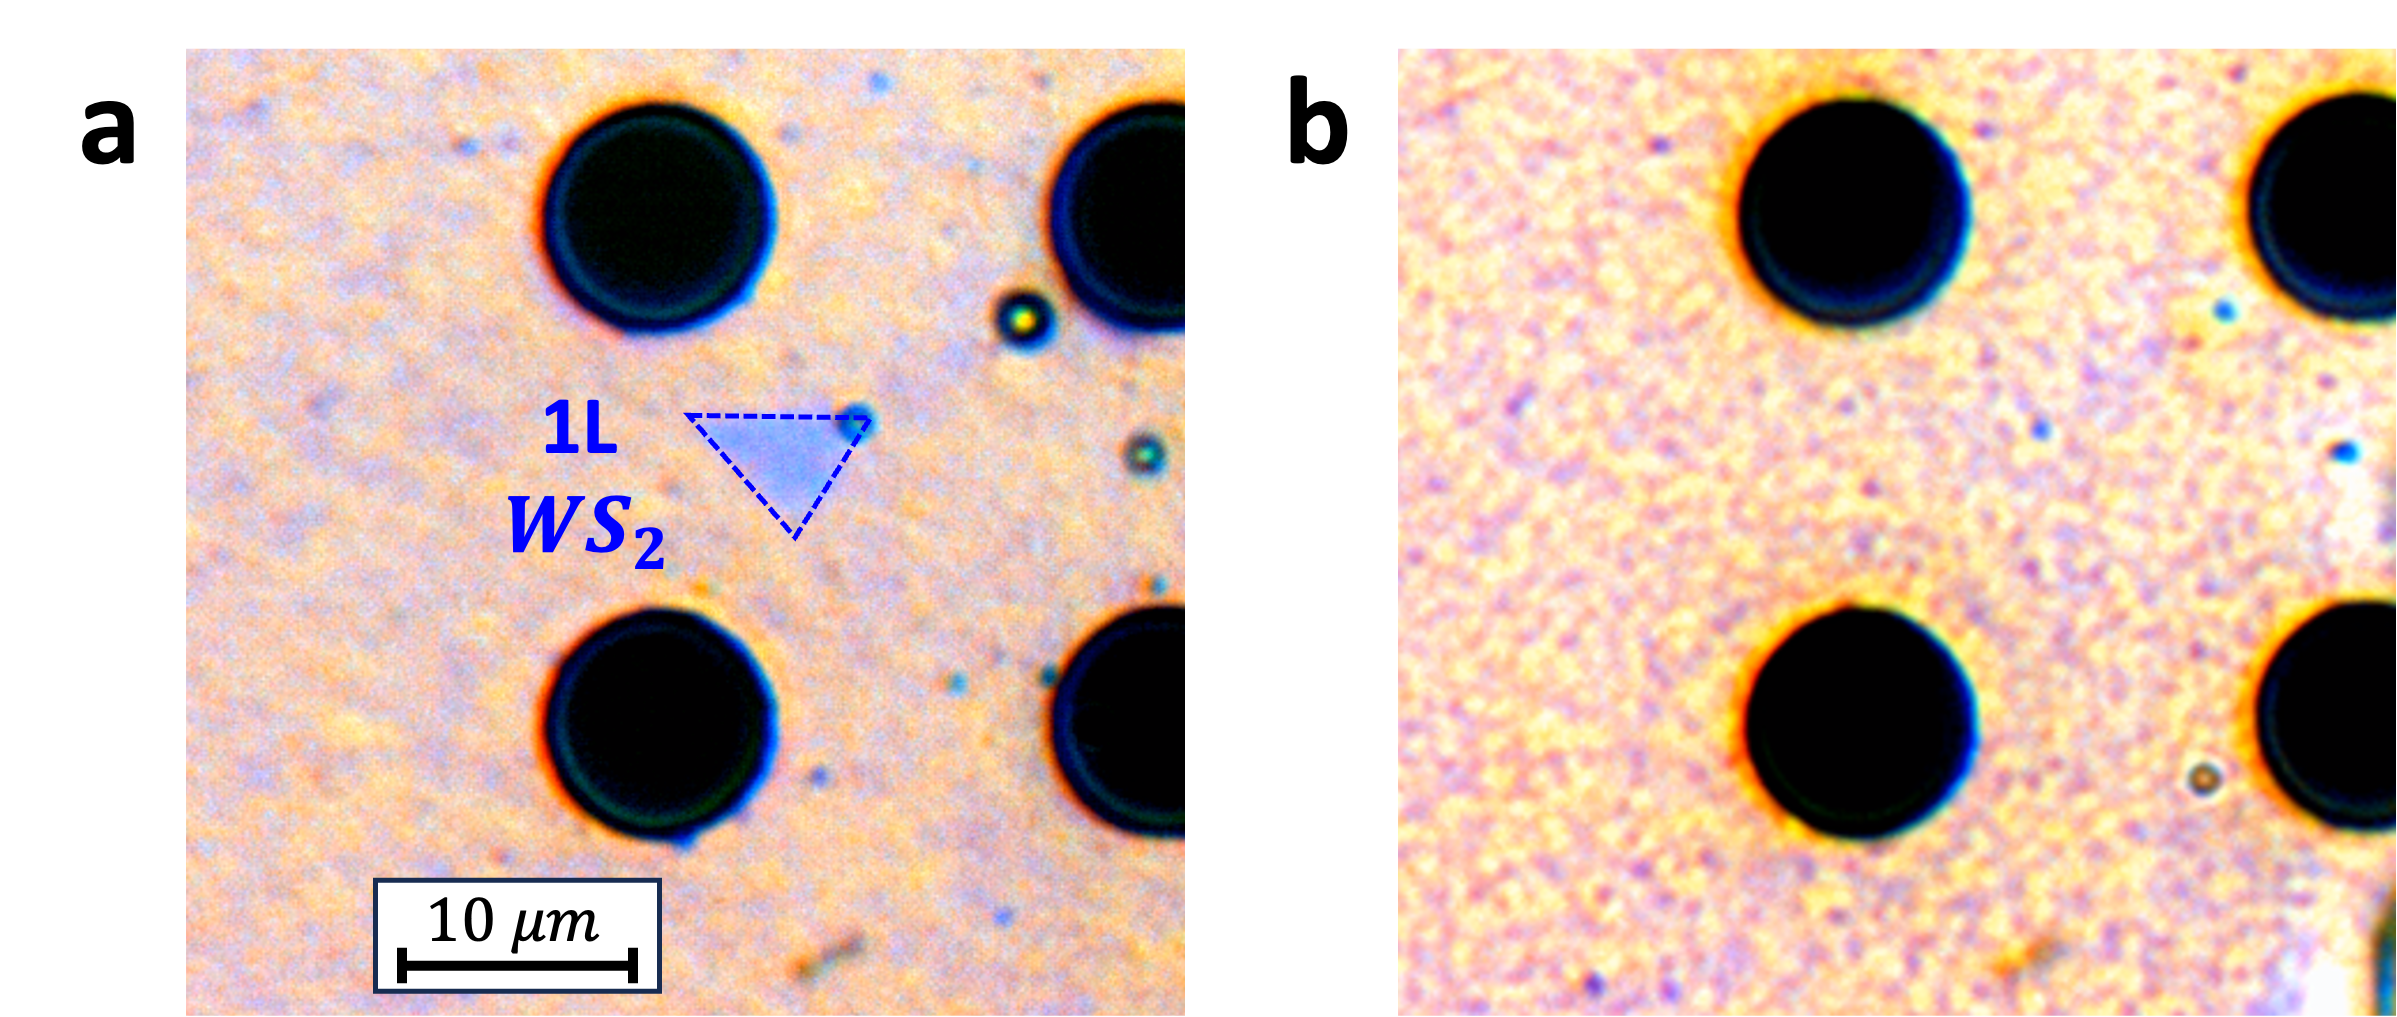
\includegraphics[width=0.9\linewidth]{Figures/dissociation.png}
  \caption{Thermal dissociation of monolayer \ce{WS2}.
    Optical images of the SiC membrane (a) before annealing, showing an
    exfoliated \ce{WS2} monolayer flake (dashed outline), and (b) after
    annealing to 1000~$^\circ$C. The \ce{WS2} monolayer is no longer visible,
    confirming thermal dissociation near 1273~K through loss of sulfur species.}
  \label{fig:s6}
\end{figure}

%%%%%%%%%%%%%%%%%%%%%%%%%%%%%%%%%%%%%%%%%%%%%%%%%%%%%%%%%%%%%%%%%%%%%
\section*{\rev{S7. Raman Intensity and Excitonic Resonances}}
%%%%%%%%%%%%%%%%%%%%%%%%%%%%%%%%%%%%%%%%%%%%%%%%%%%%%%%%%%%%%%%%%%%%%

\rev{Figure} \ref{fig:s7} \rev{shows the integrated intensity of the
E$^1_{2g}$+2LA band and the A$_{1g}$ mode versus temperature (arbitrary units,
not comparable between the two samples). The temperature dependence reflects
resonance Raman scattering} \cite{delcorro-2016}\rev{, which is strongest for
the double-resonant 2LA(M) band} \cite{berkdemir-2013}. \rev{As the excitonic
transitions redshift with temperature, the B exciton ($\sim$2.4~eV at room
temperature}~\cite{zhu-2015}\rev{) crosses the excitation energy (2.410~eV),
giving the sharp maximum near 225~K in the encapsulated sample and the maximum
at 298~K in the non-encapsulated one. The recovery of both bands above
$\sim$900~K in the encapsulated sample is attributed to the approach of the
higher-lying C exciton resonance ($\sim$2.8~eV at room
temperature}~\cite{zhu-2015}\rev{), a regime that the non-encapsulated
monolayer does not reach because it dissociates above $\sim$1223~K} (Sec.~S6).

\begin{figure}[H]
  \centering
  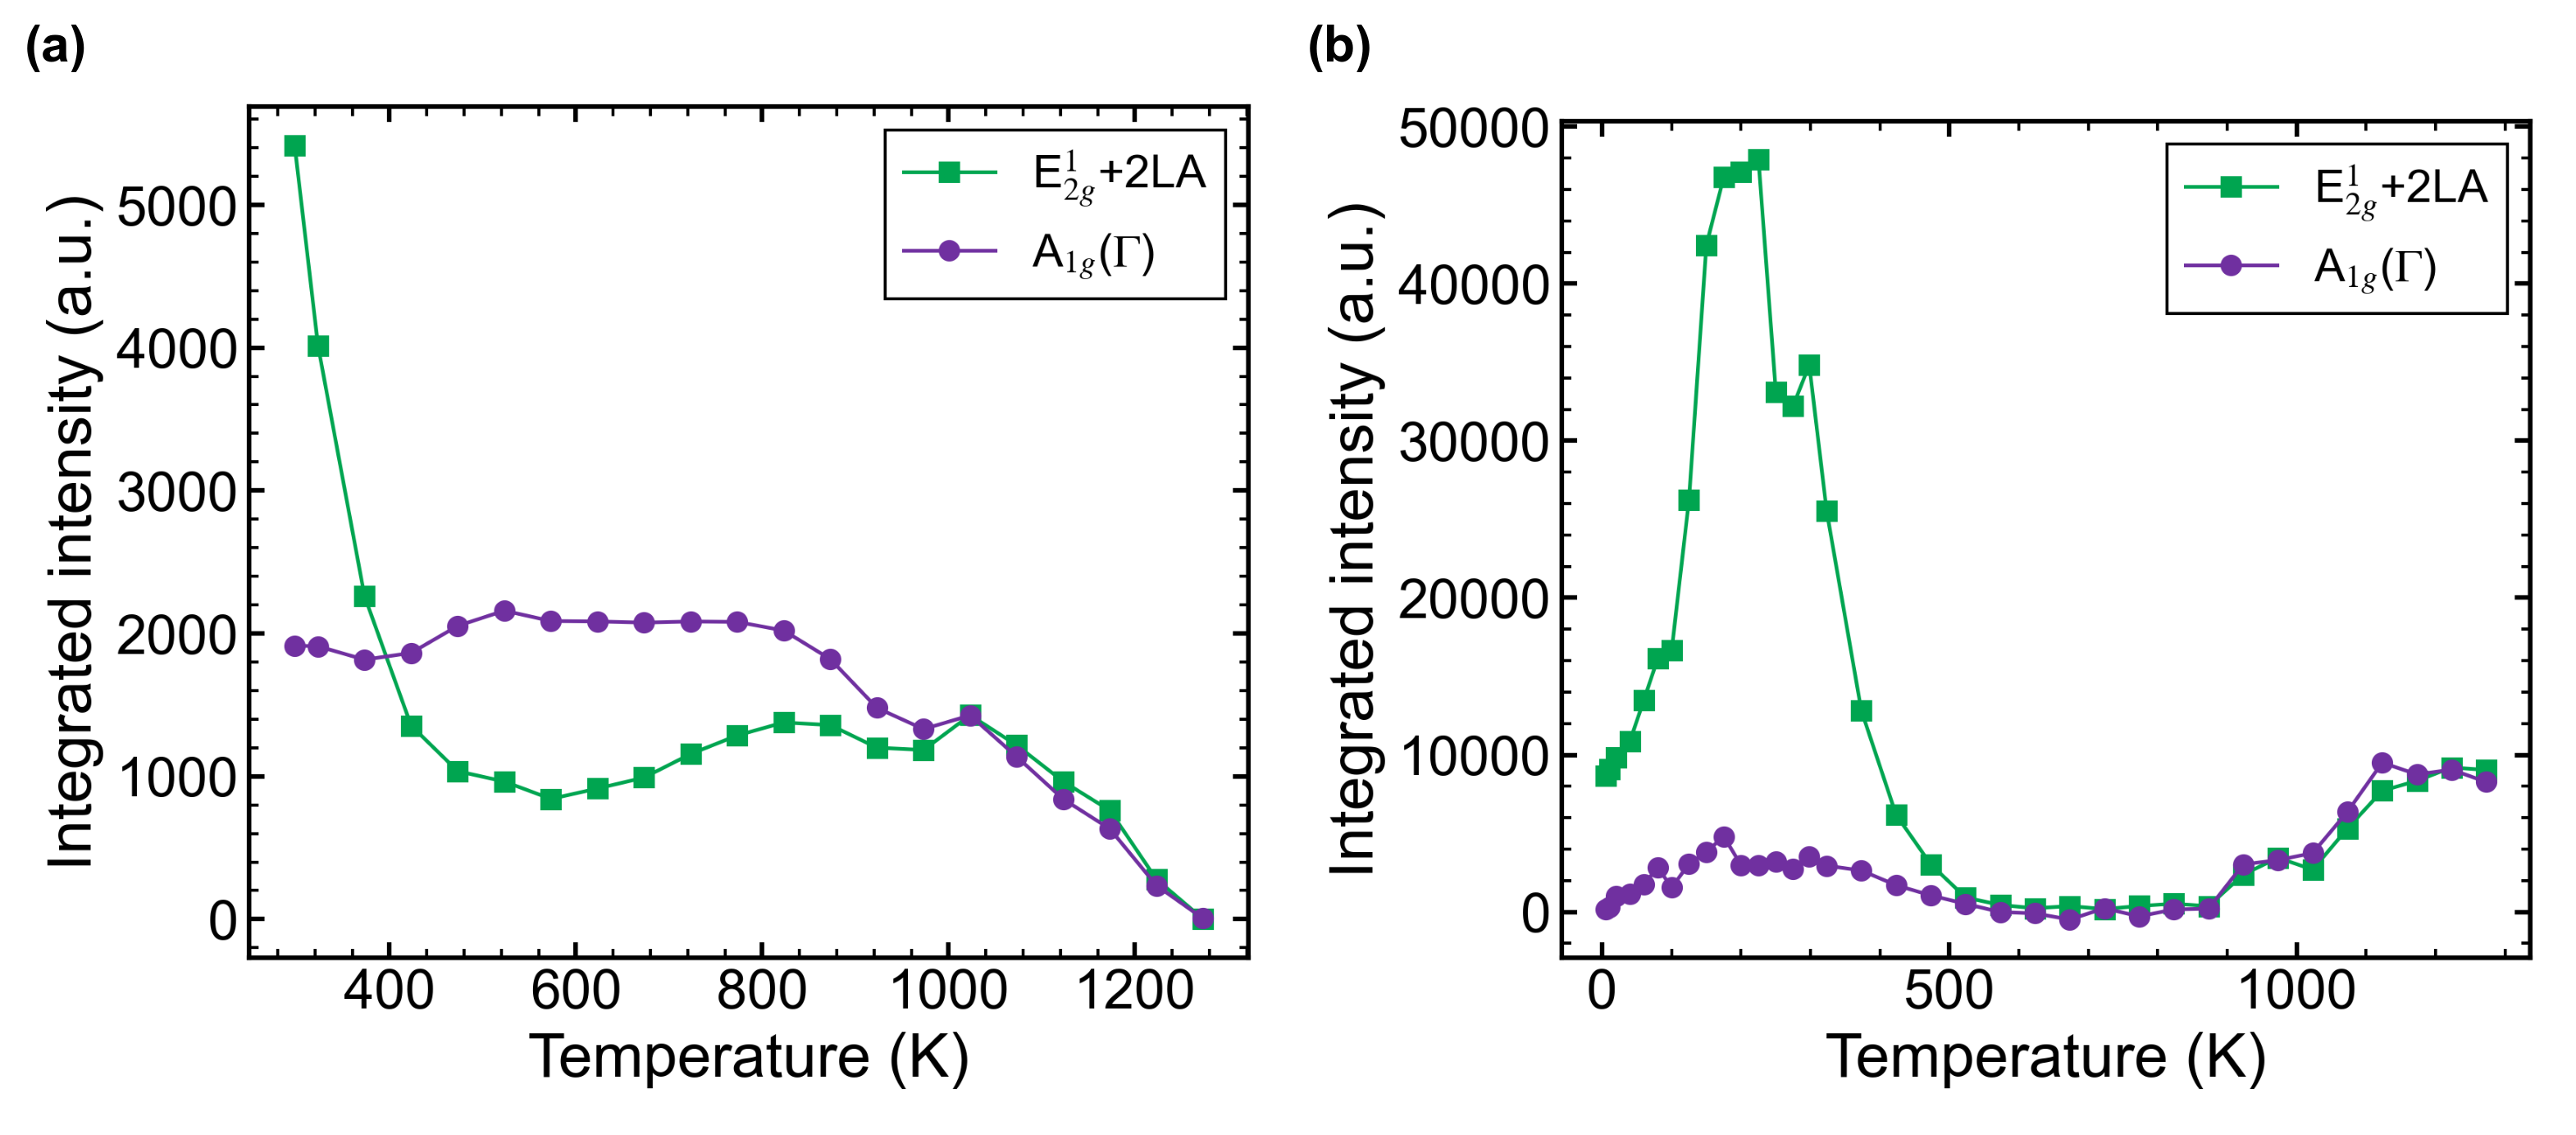
\includegraphics[width=\linewidth]{Figures/figS7.png}
  \caption{\rev{Integrated Raman intensity of the E$^1_{2g}$+2LA band (green
    squares) and the A$_{1g}$ mode (purple circles) versus temperature for (a)
    the non-encapsulated and (b) the hBN-encapsulated sample. Intensities are in
    arbitrary units and are not comparable between the two samples.}}
  \label{fig:s7}
\end{figure}

%%%%%%%%%%%%%%%%%%%%%%%%%%%%%%%%%%%%%%%%%%%%%%%%%%%%%%%%%%%%%%%%%%%%%
\printbibliography
%%%%%%%%%%%%%%%%%%%%%%%%%%%%%%%%%%%%%%%%%%%%%%%%%%%%%%%%%%%%%%%%%%%%%

\end{document}
